%%%%%%%%%%%%%%%%%%%%%%%%%%%%%%%%%%%%%%%%%%%%%%%%%%%%%%%%%%%%%%%%%%%%%%%%%%%%%%%
% CASE STUDY TEMPLATE - Programming and Problem Solving
% Author: Brendan Shea, PhD
% Course: Programming and Problem Solving
% Rochester Community and Technical College
%%%%%%%%%%%%%%%%%%%%%%%%%%%%%%%%%%%%%%%%%%%%%%%%%%%%%%%%%%%%%%%%%%%%%%%%%%%%%%%

\documentclass[11pt,letterpaper]{article}

%---------- PACKAGES ----------%
\usepackage[margin=1in, headheight=22pt]{geometry}
\usepackage[T1]{fontenc}
\usepackage{xcolor}
\usepackage{tcolorbox}
\usepackage{graphicx}
\usepackage{titlesec}
\usepackage{enumitem}
\usepackage{fancyhdr}
\usepackage{listings}
\usepackage{hyperref}
\usepackage{multicol}
\usepackage{booktabs}
\usepackage{tikz}
\usepackage{float}

% TikZ libraries
\usetikzlibrary{shapes.geometric, arrows.meta, positioning, calc, backgrounds, fit, matrix, decorations.pathreplacing}

% Load tcolorbox libraries
\tcbuselibrary{skins,breakable,listings,listingsutf8}

%---------- COLOR DEFINITIONS ----------%
\definecolor{csprimary}{HTML}{2C3E50}
\definecolor{cssecondary}{HTML}{E74C3C}
\definecolor{cstertiary}{HTML}{3498DB}
\definecolor{csaccent}{HTML}{27AE60}
\definecolor{cswarm}{HTML}{F39C12}
\definecolor{cslight}{HTML}{ECF0F1}
\definecolor{csdark}{HTML}{1A252F}

% Syntax highlighting colors
\definecolor{codegreen}{HTML}{27AE60}
\definecolor{codepurple}{HTML}{9B59B6}
\definecolor{codeorange}{HTML}{E67E22}
\definecolor{codeblue}{HTML}{3498DB}
\definecolor{codegray}{HTML}{95A5A6}
\definecolor{codestring}{HTML}{E74C3C}
\definecolor{codebg}{HTML}{1E2A38}

%---------- CASE STUDY METADATA ----------%
\newcommand{\cstitle}{Six Ways to Store Nothing}
\newcommand{\cssubtitle}{What Zero Teaches Us About Data Types}
\newcommand{\csauthor}{Brendan Shea, PhD}
\newcommand{\cscourse}{Programming and Problem Solving}
\newcommand{\csinstitution}{Rochester Community and Technical College}
\newcommand{\csdate}{\today}

%---------- LISTINGS CONFIGURATION ----------%
\lstdefinestyle{basestyle}{
    backgroundcolor=\color{codebg},
    basicstyle=\ttfamily\small\color{white},
    breakatwhitespace=false,
    breaklines=true,
    captionpos=b,
    keepspaces=true,
    showspaces=false,
    showstringspaces=false,
    showtabs=false,
    tabsize=4,
    frame=none,
    xleftmargin=4mm,
    xrightmargin=4mm,
    aboveskip=0pt,
    belowskip=0pt,
}

\lstdefinestyle{javastyle}{
    style=basestyle,
    language=Java,
    keywordstyle=\color{codeblue}\bfseries,
    commentstyle=\color{codegray}\itshape,
    stringstyle=\color{codestring},
    morekeywords={String, Scanner, System, var},
}

%---------- CUSTOM ENVIRONMENTS ----------%
\newcommand{\keyterm}[1]{\textbf{\textcolor{cssecondary}{#1}}}

\newtcolorbox{conceptbox}[1][]{
    enhanced,
    colback=cslight,
    colframe=csprimary,
    fonttitle=\bfseries\color{white},
    title=#1,
    attach boxed title to top left={yshift=-2mm, xshift=5mm},
    boxed title style={colback=csprimary},
    breakable
}

\newtcolorbox{historybox}[1][]{
    enhanced,
    colback=codepurple!8,
    colframe=codepurple,
    fonttitle=\bfseries\color{white},
    title=#1,
    attach boxed title to top left={yshift=-2mm, xshift=5mm},
    boxed title style={colback=codepurple},
    breakable
}

\newtcolorbox{codebox}[2][]{
    enhanced,
    colback=codebg,
    colframe=csaccent,
    colupper=white,
    fonttitle=\bfseries\color{white},
    title=#2,
    attach boxed title to top left={yshift=-2mm, xshift=5mm},
    boxed title style={colback=csaccent},
    left=0mm, right=0mm, top=2mm, bottom=2mm,
    boxrule=1pt,
    breakable,
    pad at break=2mm,
    #1
}

\newtcblisting{javacode}[1][]{
    enhanced,
    colback=codebg,
    colframe=csaccent,
    colupper=white,
    fonttitle=\bfseries\color{white},
    title=#1,
    attach boxed title to top left={yshift=-2mm, xshift=5mm},
    boxed title style={colback=csaccent},
    left=0mm, right=0mm, top=2mm, bottom=2mm,
    boxrule=1pt,
    breakable,
    pad at break=2mm,
    listing only,
    listing options={style=javastyle}
}

\newtcolorbox{questionbox}{
    enhanced,
    colback=cswarm!10,
    colframe=cswarm,
    fonttitle=\bfseries\color{white},
    title=Discussion Questions,
    attach boxed title to top center={yshift=-2mm},
    boxed title style={colback=cswarm},
    breakable
}

\newtcolorbox{glossarybox}{
    enhanced,
    colback=cslight,
    colframe=csprimary,
    fonttitle=\bfseries\color{white},
    title=Glossary of Key Terms,
    attach boxed title to top center={yshift=-2mm},
    boxed title style={colback=csprimary},
    breakable
}

%---------- HEADER/FOOTER ----------%
\pagestyle{fancy}
\fancyhf{}
\fancyhead[L]{\small\textcolor{csprimary}{\cscourse}}
\fancyhead[R]{\small\textcolor{csprimary}{Case Study}}
\fancyfoot[C]{\thepage}
\renewcommand{\headrulewidth}{0.4pt}
\renewcommand{\headrule}{\hbox to\headwidth{\color{csprimary}\leaders\hrule height \headrulewidth\hfill}}

%---------- SECTION FORMATTING ----------%
\titleformat{\section}
    {\Large\bfseries\color{csprimary}}
    {\thesection}{1em}{}[\color{cssecondary}\titlerule]
    
\titleformat{\subsection}
    {\large\bfseries\color{cstertiary}}
    {\thesubsection}{1em}{}

%---------- HYPERLINK SETTINGS ----------%
\hypersetup{
    colorlinks=true,
    linkcolor=cstertiary,
    urlcolor=cstertiary
}

%%%%%%%%%%%%%%%%%%%%%%%%%%%%%%%%%%%%%%%%%%%%%%%%%%%%%%%%%%%%%%%%%%%%%%%%%%%%%%%
\begin{document}

%---------- TITLE BLOCK ----------%
\begin{tcolorbox}[
    enhanced,
    colback=csprimary,
    colframe=csprimary,
    arc=0mm,
    left=10mm, right=10mm, top=8mm, bottom=8mm
]
\begin{center}
    {\huge\bfseries\color{white}\cstitle}\\[3mm]
    {\Large\color{cslight}\cssubtitle}\\[5mm]
    \textcolor{cssecondary}{\rule{0.5\textwidth}{1pt}}\\[5mm]
    {\large\color{white}\csauthor}\\[2mm]
    {\normalsize\color{cslight}\cscourse\ $\bullet$ \csinstitution}
\end{center}
\end{tcolorbox}

\vspace{5mm}

%---------- INTRODUCTION ----------%
\section*{Introduction}

Zero seems simple. It's nothing, right? But in programming, ``nothing'' turns out to be surprisingly complicated. Consider these six Java declarations:

\begin{javacode}[Six Ways to Store ``Zero'']
int a = 0;           // An integer zero
double b = 0.0;      // A floating-point zero
char c = '0';        // The character zero
String d = "0";      // A string containing zero
boolean e = false;   // A boolean "zero" (false)
int[] f = {0};       // An array containing one zero
\end{javacode}

Each of these represents ``zero'' in some sense, yet the computer stores each one completely differently. Understanding \textit{why} requires us to peek beneath Java's surface and see how computers actually represent information. This journey will illuminate one of programming's most fundamental concepts: \keyterm{data types} aren't just arbitrary rules---they reflect deep truths about how computers work with information, and decades of hard-won engineering wisdom.

\begin{conceptbox}[The Central Question]
If a computer only understands 1s and 0s, how does it know whether \texttt{01000000} means the number 64, the character `@', or something else entirely? The answer reveals why data types exist and why they matter.
\end{conceptbox}

%---------- BINARY FOUNDATION ----------%
\section{The Binary Foundation}

Every piece of data in a computer---every number, letter, image, and sound---is ultimately stored as a sequence of \keyterm{bits}. A bit is the smallest unit of information: it can be either 0 or 1, like a tiny light switch that's either off or on. Why binary? Because electronic circuits can reliably distinguish between two states (high voltage vs.\ low voltage, charged vs.\ uncharged) far more easily than multiple states. This physical reality shapes everything in computing.

Eight bits grouped together form a \keyterm{byte}, which can represent $2^8 = 256$ different values (from 00000000 to 11111111).

\begin{center}
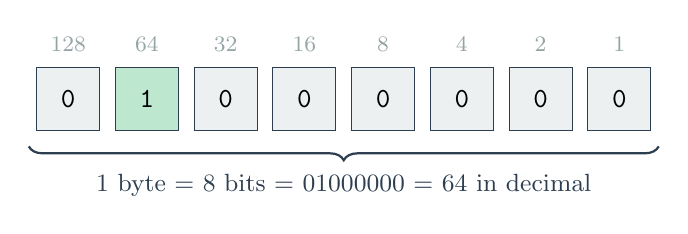
\begin{tikzpicture}[
    bit/.style={rectangle, draw=csprimary, fill=#1, minimum width=8mm, minimum height=8mm, font=\ttfamily\bfseries},
    label/.style={font=\footnotesize\color{codegray}}
]
% One byte showing 01000000
\node[bit=cslight] (b7) at (0,0) {0};
\node[bit=csaccent!30] (b6) at (1,0) {1};
\node[bit=cslight] (b5) at (2,0) {0};
\node[bit=cslight] (b4) at (3,0) {0};
\node[bit=cslight] (b3) at (4,0) {0};
\node[bit=cslight] (b2) at (5,0) {0};
\node[bit=cslight] (b1) at (6,0) {0};
\node[bit=cslight] (b0) at (7,0) {0};

% Bit position labels
\node[label] at (0,0.7) {128};
\node[label] at (1,0.7) {64};
\node[label] at (2,0.7) {32};
\node[label] at (3,0.7) {16};
\node[label] at (4,0.7) {8};
\node[label] at (5,0.7) {4};
\node[label] at (6,0.7) {2};
\node[label] at (7,0.7) {1};

% Bracket and label
\draw[decorate, decoration={brace, amplitude=5pt, mirror}, thick, csprimary] 
    (-0.5,-0.6) -- (7.5,-0.6);
\node[font=\small, color=csprimary] at (3.5,-1.1) {1 byte = 8 bits = 01000000 = 64 in decimal};

\end{tikzpicture}
\end{center}

But here's the crucial insight: the bit pattern \texttt{01000000} is \textit{just a pattern}. By itself, it has no inherent meaning. It could represent the integer 64, or the character `@' (whose \keyterm{ASCII} code is 64), or part of a larger number, or something else entirely. The \keyterm{data type} is what tells the computer---and other programmers---how to interpret the pattern.

%---------- INTEGER ZERO ----------%
\section{Integer Zero: \texttt{int a = 0}}

When you declare \texttt{int a = 0} in Java, you're asking the computer to reserve 32 bits (4 bytes) of memory and store the integer value zero. For positive integers, computers use \keyterm{binary representation}---the same place-value system we use for decimal numbers, but with powers of 2 instead of powers of 10.

Integer zero is simple: all 32 bits are 0. But what about negative numbers? You might think we could just use one bit as a ``sign bit'' (0 for positive, 1 for negative) and keep the rest the same. Early computers tried this, but it created problems: you'd have both ``positive zero'' and ``negative zero,'' and arithmetic circuits became complicated.

\subsection{Two's Complement: A Clever Solution}

Java, like virtually all modern computers, uses \keyterm{two's complement} to represent negative integers. This system has an elegant property: the same electronic circuits that add positive numbers automatically handle negative numbers correctly.

\begin{center}
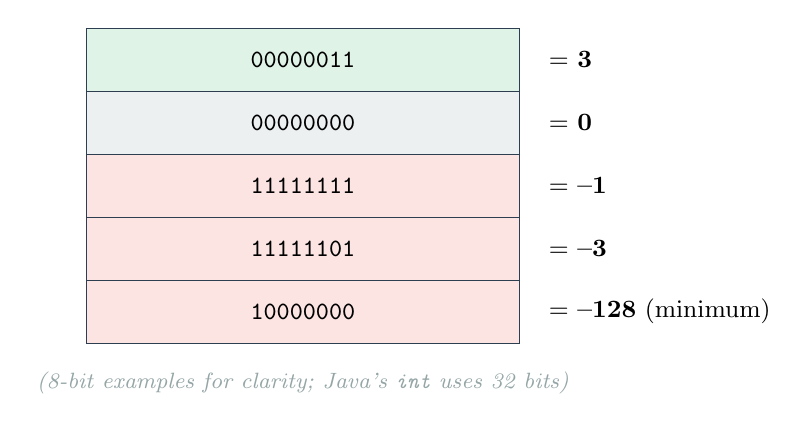
\begin{tikzpicture}[
    numbox/.style={rectangle, draw=csprimary, fill=#1, minimum width=55mm, minimum height=8mm, font=\ttfamily\small, align=left},
    label/.style={font=\small}
]
% Examples with 8 bits for clarity
\node[numbox=csaccent!15] (p3) at (0,1.6) { 00000011};
\node[label, anchor=west] at (3,1.6) {= \textbf{3}};

\node[numbox=cslight] (z) at (0,0.8) { 00000000};
\node[label, anchor=west] at (3,0.8) {= \textbf{0}};

\node[numbox=cssecondary!15] (n1) at (0,0) { 11111111};
\node[label, anchor=west] at (3,0) {= \textbf{--1}};

\node[numbox=cssecondary!15] (n3) at (0,-0.8) { 11111101};
\node[label, anchor=west] at (3,-0.8) {= \textbf{--3}};

\node[numbox=cssecondary!15] (min) at (0,-1.6) { 10000000};
\node[label, anchor=west] at (3,-1.6) {= \textbf{--128} (minimum)};

% Note
\node[font=\footnotesize\itshape, color=codegray, align=center] at (0,-2.5) {(8-bit examples for clarity; Java's \texttt{int} uses 32 bits)};

\end{tikzpicture}
\end{center}

Notice the pattern: positive numbers start with 0, negative numbers start with 1. But it's not a simple sign bit---the value $-1$ is represented as all 1s, not as a 1 followed by the pattern for 1. The ``two's complement'' of a number is found by flipping all bits and adding 1. This seems strange, but it makes addition work seamlessly: if you add the bit patterns for 3 and $-1$ using ordinary binary addition, you get 2. The circuits don't need to know whether they're adding positive or negative numbers.

This design also explains a quirk: with 32 bits, Java's \texttt{int} can represent values from $-2,147,483,648$ to $+2,147,483,647$. Notice there's one more negative value than positive---that's because zero takes one of the ``positive'' slots.

%---------- FLOATING POINT ZERO ----------%
\section{Floating-Point Zero: \texttt{double b = 0.0}}

Integers are great for counting, but what about measurements, currencies, or scientific calculations that need decimal points? For these, we need \keyterm{floating-point} numbers---but their story involves one of computing's most important standardization efforts.

\begin{historybox}[Why We Needed a Standard: The Floating-Point Wars]
In the 1970s, different computer manufacturers used different floating-point formats. A program that worked correctly on an IBM mainframe might give wrong answers on a DEC minicomputer. Scientific calculations couldn't be trusted across different machines. Financial software was a nightmare.

In 1985, the Institute of Electrical and Electronics Engineers (IEEE) published standard 754, defining exactly how floating-point numbers should be stored and how arithmetic should work. The effort was led by Professor William Kahan, who later won computing's highest honor (the Turing Award) partly for this work. Today, virtually every computer, phone, and calculator follows IEEE 754---including Java.
\end{historybox}

A \texttt{double} uses 64 bits divided into three parts, similar to scientific notation. Just as we write $6.02 \times 10^{23}$ for Avogadro's number (with a sign, a ``significand'' of 6.02, and an exponent of 23), floating-point stores:

\begin{center}
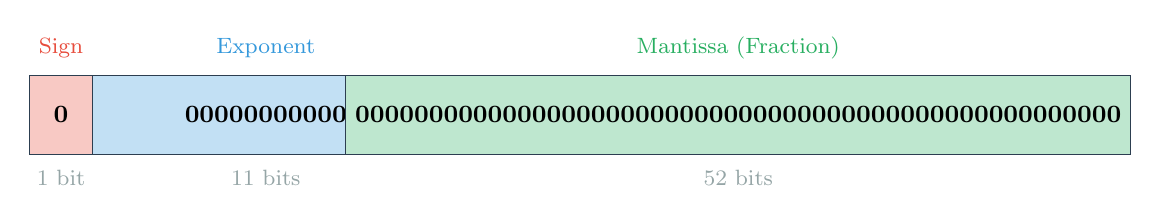
\begin{tikzpicture}[
    section/.style={rectangle, draw=csprimary, fill=#1, minimum height=10mm, font=\small\bfseries},
    label/.style={font=\footnotesize}
]
% Sign bit
\node[section=cssecondary!30, minimum width=8mm] (sign) at (0,0) {0};
\node[label, color=cssecondary] at (0,0.85) {Sign};
\node[label, color=codegray] at (0,-0.8) {1 bit};

% Exponent
\node[section=cstertiary!30, minimum width=44mm] (exp) at (2.6,0) {00000000000};
\node[label, color=cstertiary] at (2.6,0.85) {Exponent};
\node[label, color=codegray] at (2.6,-0.8) {11 bits};

% Mantissa
\node[section=csaccent!30, minimum width=80mm] (mant) at (8.6,0) {0000000000000000000000000000000000000000000000000000};
\node[label, color=csaccent] at (8.6,0.85) {Mantissa (Fraction)};
\node[label, color=codegray] at (8.6,-0.8) {52 bits};

\end{tikzpicture}
\end{center}

This design lets \texttt{double} represent both the astronomically large ($\approx 10^{308}$) and the infinitesimally small ($\approx 10^{-308}$). For zero, all 64 bits are 0---though IEEE 754 actually defines both positive zero (\texttt{+0.0}) and negative zero (\texttt{-0.0}), which compare as equal but can arise from different calculations.

\subsection{The Price of Flexibility}

Floating-point's flexibility comes with an important trade-off: most decimal numbers cannot be represented \textit{exactly}. Just as $\frac{1}{3} = 0.333...$ goes on forever in decimal, the simple value $0.1$ goes on forever in binary. The computer stores the closest approximation it can fit in 64 bits.

This is why \texttt{0.1 + 0.2 == 0.3} returns \texttt{false} in Java---the tiny rounding errors don't cancel out. Programs dealing with money often use integers (counting cents rather than fractional dollars) or special classes like \texttt{BigDecimal} to avoid these surprises.

%---------- CHARACTER ZERO ----------%
\section{Character Zero: \texttt{char c = '0'}}

When you write \texttt{char c = '0'}, you're not storing the number zero at all. You're storing the \textit{character} that looks like zero---the symbol we write when we want to display the digit. In Java, a \texttt{char} uses 16 bits to store a \keyterm{Unicode} value.

\begin{center}
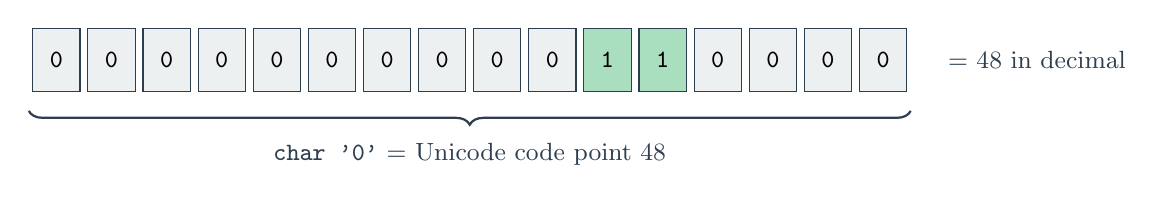
\begin{tikzpicture}[
    bit/.style={rectangle, draw=csprimary, fill=#1, minimum width=6mm, minimum height=8mm, font=\ttfamily\small},
]
% 16 bits for '0' = Unicode 48 = 0000000000110000
\node[bit=cslight] at (0,0) {0};
\node[bit=cslight] at (0.7,0) {0};
\node[bit=cslight] at (1.4,0) {0};
\node[bit=cslight] at (2.1,0) {0};
\node[bit=cslight] at (2.8,0) {0};
\node[bit=cslight] at (3.5,0) {0};
\node[bit=cslight] at (4.2,0) {0};
\node[bit=cslight] at (4.9,0) {0};
\node[bit=cslight] at (5.6,0) {0};
\node[bit=cslight] at (6.3,0) {0};
\node[bit=csaccent!40] at (7.0,0) {1};
\node[bit=csaccent!40] at (7.7,0) {1};
\node[bit=cslight] at (8.4,0) {0};
\node[bit=cslight] at (9.1,0) {0};
\node[bit=cslight] at (9.8,0) {0};
\node[bit=cslight] at (10.5,0) {0};

\node[font=\small, color=csprimary, anchor=west] at (11.2,0) {= 48 in decimal};

\draw[decorate, decoration={brace, amplitude=5pt, mirror}, thick, csprimary] 
    (-0.35,-0.65) -- (10.85,-0.65);
\node[font=\small, color=csprimary] at (5.25,-1.2) {\texttt{char '0'} = Unicode code point 48};
\end{tikzpicture}
\end{center}

The character `0' has Unicode value 48---so \texttt{(int)'0'} equals 48, not 0! The digit characters are arranged consecutively: `0' is 48, `1' is 49, `2' is 50, and so on up to `9' at 57. This clever arrangement means you can convert a digit character to its numeric value by subtracting `0': the expression \texttt{'7' - '0'} equals 7.

This distinction between the \textit{character} `0' and the \textit{number} 0 is fundamental. When you type ``2024'' on your keyboard, you're creating four characters. The computer must \keyterm{parse} this text---analyze it and convert it---to get the actual number 2024. That's what methods like \texttt{Integer.parseInt()} do.

%---------- STRING ZERO ----------%
\section{String Zero: \texttt{String d = "0"}}

A \texttt{String} in Java is fundamentally different from the types we've seen so far. It's an \keyterm{object}---a more complex structure that bundles data together with operations on that data.

\subsection{Why Objects? Managing Complexity}

Imagine if every time you wanted to work with text, you had to manually manage an array of characters, track its length, handle memory allocation when the text grows, and implement operations like searching and replacing from scratch. This would be tedious and error-prone.

Objects solve this by \keyterm{encapsulation}---bundling related data and operations into a single unit. A String object contains the characters, knows its own length, and provides methods like \texttt{.substring()}, \texttt{.toUpperCase()}, and \texttt{.equals()}. You don't need to know \textit{how} these work internally; you just use them.

\begin{center}
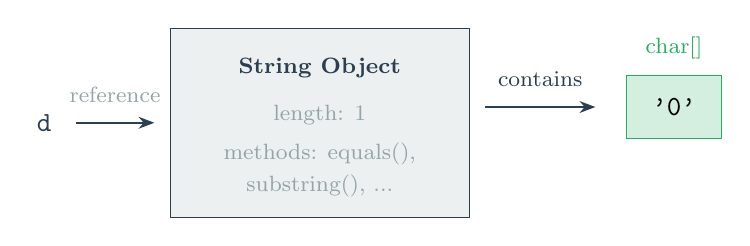
\begin{tikzpicture}[
    box/.style={rectangle, draw=csprimary, fill=cslight, minimum width=25mm, minimum height=8mm, font=\small},
    charbox/.style={rectangle, draw=csaccent, fill=csaccent!20, minimum width=12mm, minimum height=8mm, font=\ttfamily},
    arrow/.style={-{Stealth[length=2mm]}, thick, color=csprimary}
]
% String object
\node[box, minimum height=24mm, minimum width=38mm] (strobj) at (0,0) {};
\node[font=\footnotesize\bfseries, color=csprimary] at (0,0.7) {String Object};
\node[font=\footnotesize, color=codegray] at (0,0.1) {length: 1};
\node[font=\footnotesize, color=codegray] at (0,-0.4) {methods: equals(),};
\node[font=\footnotesize, color=codegray] at (0,-0.8) {substring(), ...};

% Reference arrow
\draw[arrow] (2.1,0.2) -- (3.5,0.2);
\node[font=\footnotesize, color=csprimary] at (2.8,0.55) {contains};

% Character array
\node[charbox] (char0) at (4.5,0.2) {'0'};
\node[font=\footnotesize, color=csaccent] at (4.5,0.95) {char[]};

% Variable
\node[font=\ttfamily, color=csprimary] at (-3.5,0) {d};
\draw[arrow] (-3.1,0) -- (-2.1,0);
\node[font=\footnotesize, color=codegray] at (-2.6,0.35) {reference};

\end{tikzpicture}
\end{center}

\subsection{References: Indirection for Flexibility}

The variable \texttt{d} doesn't actually contain the string data---it contains a \keyterm{reference}, essentially the memory address where the String object lives. This indirection exists for good reasons: strings can be any length, from empty to millions of characters. If variables had to contain the actual data, the compiler couldn't know how much space to reserve. References are always the same size (typically 32 or 64 bits), regardless of what they point to.

This is why comparing strings with \texttt{==} can be misleading---you're comparing whether two references point to the \textit{same object}, not whether two objects contain the \textit{same characters}. The \texttt{.equals()} method compares content.

%---------- BOOLEAN ZERO ----------%
\section{Boolean ``Zero'': \texttt{boolean e = false}}

The \keyterm{boolean} type represents logical truth values: \texttt{true} or \texttt{false}. In a sense, \texttt{false} is the ``zero'' of logic---the absence of truth, the negative case, the condition that fails.

\begin{center}
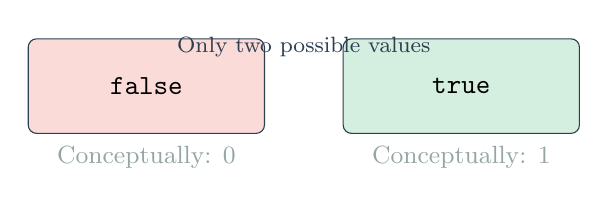
\begin{tikzpicture}[
    box/.style={rectangle, rounded corners=3pt, draw=csprimary, fill=#1, minimum width=30mm, minimum height=12mm, font=\bfseries},
]
\node[box=cssecondary!20] (false) at (0,0) {\texttt{false}};
\node[box=csaccent!20] (true) at (4,0) {\texttt{true}};

\node[font=\small, color=codegray] at (0,-0.9) {Conceptually: 0};
\node[font=\small, color=codegray] at (4,-0.9) {Conceptually: 1};

\node[font=\footnotesize, color=csprimary] at (2,0.5) {Only two possible values};
\end{tikzpicture}
\end{center}

While a boolean conceptually needs only 1 bit, Java doesn't specify exactly how it's stored---the JVM might use a full byte for efficiency, since modern computers access memory in byte-sized chunks.

Some languages (like C, Python, and JavaScript) treat 0 as ``falsy'' and nonzero values as ``truthy,'' allowing code like \texttt{if (count)} instead of \texttt{if (count != 0)}. Java deliberately forbids this. Why? Because mixing numeric and logical operations is a common source of bugs. If \texttt{x = 5} (assignment) were allowed in a condition, typos could silently corrupt your program. Java's strictness catches these errors at compile time.

%---------- ARRAY ZERO ----------%
\section{An Array of Zero: \texttt{int[] f = \{0\}}}

An \keyterm{array} is a container that holds multiple values of the same type, stored consecutively in memory. When you write \texttt{int[] f = \{0\}}, you create an array holding exactly one integer (which happens to be zero).

\subsection{Why Arrays? Efficiency and Structure}

Imagine tracking scores for 100 students. Without arrays, you'd need 100 separate variables: \texttt{score1}, \texttt{score2}, ... \texttt{score100}. You couldn't easily loop through them or pass them to a method as a group.

Arrays solve this by storing elements consecutively in memory. Because each \texttt{int} is exactly 32 bits, the computer can instantly calculate where element $n$ is stored: it's at the array's starting address plus $n \times 4$ bytes. This \keyterm{random access}---jumping directly to any element---takes the same amount of time whether you want element 0 or element 999,999.

\begin{center}
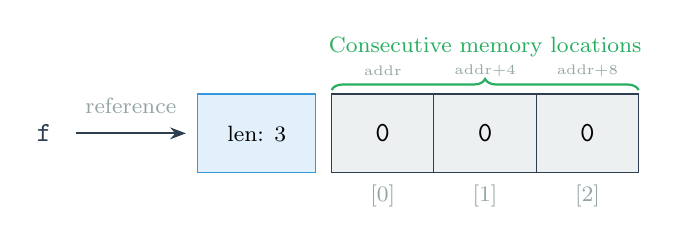
\begin{tikzpicture}[
    cell/.style={rectangle, draw=csprimary, fill=cslight, minimum width=13mm, minimum height=10mm, font=\ttfamily},
    idx/.style={font=\footnotesize\color{codegray}},
    arrow/.style={-{Stealth[length=2mm]}, thick, color=csprimary}
]
% Variable f
\node[font=\ttfamily, color=csprimary] (fvar) at (-1.5,0) {f};

% Reference arrow
\draw[arrow] (-1.1,0) -- (0.3,0);
\node[font=\footnotesize\color{codegray}] at (-0.4,0.35) {reference};

% Array header
\node[rectangle, draw=cstertiary, fill=cstertiary!15, minimum width=15mm, minimum height=10mm, font=\footnotesize] (len) at (1.2,0) {len: 3};

% Array cells
\node[cell] (c0) at (2.8,0) {0};
\node[cell] (c1) at (4.1,0) {0};
\node[cell] (c2) at (5.4,0) {0};

\node[idx] at (2.8,-0.8) {[0]};
\node[idx] at (4.1,-0.8) {[1]};
\node[idx] at (5.4,-0.8) {[2]};

% Memory addresses hint
\node[font=\tiny\color{codegray}] at (2.8,0.8) {addr};
\node[font=\tiny\color{codegray}] at (4.1,0.8) {addr+4};
\node[font=\tiny\color{codegray}] at (5.4,0.8) {addr+8};

\draw[decorate, decoration={brace, amplitude=4pt}, thick, csaccent] 
    (2.15,0.55) -- (6.05,0.55);
\node[font=\footnotesize, color=csaccent] at (4.1,1.1) {Consecutive memory locations};

\end{tikzpicture}
\end{center}

Like strings, arrays are objects accessed by reference. The array knows its own length (which cannot change after creation), and Java checks every access to prevent reading or writing beyond the array's bounds---a major source of security vulnerabilities in languages like C.

When you create an array with \texttt{new int[10]}, Java automatically initializes all elements to zero. This \keyterm{default initialization} prevents you from accidentally reading garbage data that happened to be in memory.

%---------- THE BIG PICTURE ----------%
\section{The Big Picture: Why Types Matter}

\begin{center}
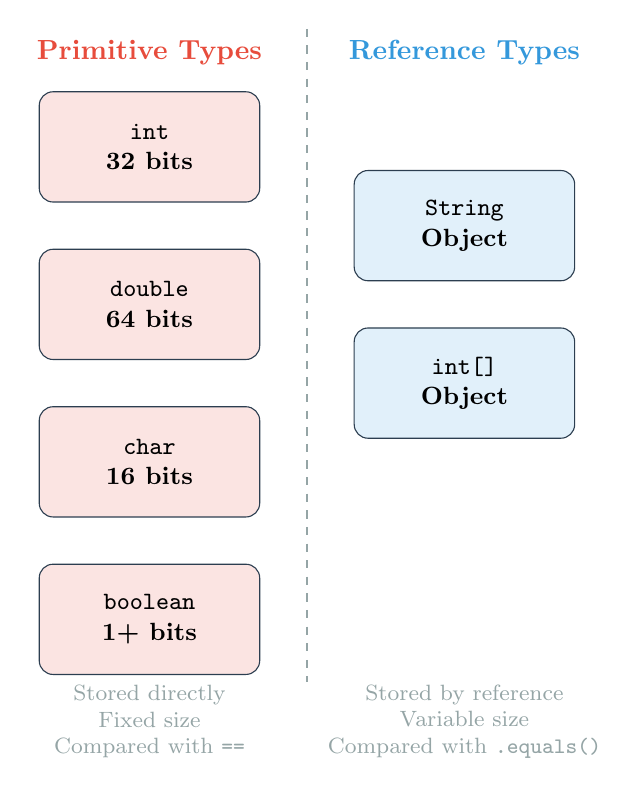
\begin{tikzpicture}[
    node distance=1.5cm,
    typebox/.style={rectangle, rounded corners=5pt, draw=csprimary, fill=#1, 
                    minimum width=28mm, minimum height=14mm, font=\small\bfseries, align=center},
]

% Primitives column
\node[typebox=cssecondary!15] (int) at (0,2) {\texttt{int}\\32 bits};
\node[typebox=cssecondary!15] (double) at (0,0) {\texttt{double}\\64 bits};
\node[typebox=cssecondary!15] (char) at (0,-2) {\texttt{char}\\16 bits};
\node[typebox=cssecondary!15] (bool) at (0,-4) {\texttt{boolean}\\1+ bits};

% Objects column
\node[typebox=cstertiary!15] (string) at (4,1) {\texttt{String}\\Object};
\node[typebox=cstertiary!15] (array) at (4,-1) {\texttt{int[]}\\Object};

% Labels
\node[font=\bfseries\color{cssecondary}] at (0,3.2) {Primitive Types};
\node[font=\bfseries\color{cstertiary}] at (4,3.2) {Reference Types};

% Dividing line
\draw[dashed, thick, color=codegray] (2,3.5) -- (2,-4.8);

% Characteristics
\node[font=\footnotesize\color{codegray}, align=center] at (0,-5.3) {Stored directly\\Fixed size\\Compared with \texttt{==}};
\node[font=\footnotesize\color{codegray}, align=center] at (4,-5.3) {Stored by reference\\Variable size\\Compared with \texttt{.equals()}};

\end{tikzpicture}
\end{center}

Our journey through six zeros reveals a fundamental divide in Java: \keyterm{primitive types} versus \keyterm{reference types}. Primitives (\texttt{int}, \texttt{double}, \texttt{char}, \texttt{boolean}) store values directly and have fixed, known sizes. Reference types (\texttt{String}, arrays, and all other objects) store references to data elsewhere in memory, allowing for variable sizes and complex structures.

Ultimately, data types exist because \textit{meaning requires context}. The same bit pattern can represent completely different things depending on interpretation. Types encode the rules---what operations make sense (you can add integers, but not booleans), what values are legal (a \texttt{boolean} can't be 7), and how comparisons work. These rules catch errors early, before they corrupt your data or crash your program at runtime.

The next time you declare a variable, remember: you're not just giving something a name. You're telling the computer---and every programmer who reads your code---exactly what kind of information you're working with and how it should be treated.

%---------- DISCUSSION QUESTIONS ----------%
\section*{Discussion Questions}

\begin{questionbox}
\begin{enumerate}[leftmargin=*, label=\textcolor{cswarm}{\textbf{\arabic*.}}]
    \item \textbf{Two's Complement Trade-offs:} In two's complement, the range of a 32-bit \texttt{int} is asymmetric: $-2,147,483,648$ to $+2,147,483,647$. What happens if you compute \texttt{Integer.MAX\_VALUE + 1}? Why might the designers have accepted this quirk rather than using a simpler sign-bit approach?

    \item \textbf{Floating-Point Pitfalls:} The expression \texttt{0.1 + 0.2 == 0.3} evaluates to \texttt{false} in Java (try it!). Given that IEEE 754 was designed by experts, why does this ``bug'' exist? How might programmers work around it for financial calculations where exactness matters?

    \item \textbf{Characters and Numbers:} The expression \texttt{'0' + 1} equals 49 (an integer), but \texttt{"0" + 1} equals \texttt{"01"} (a String). Why do these similar-looking expressions behave so differently? What rules is Java following?

    \item \textbf{The Value of Standards:} Before IEEE 754, the same program could give different numerical results on different computers. What are the benefits of having a universal standard, even if that standard has known limitations (like the 0.1 + 0.2 problem)? Can you think of other areas of computing or life where standardization matters?

    \item \textbf{Null: The Seventh Zero?} Java has another way to represent ``nothing'': the special value \texttt{null}, which means ``this reference points to no object.'' How is \texttt{null} different from an empty string \texttt{""} or an array of length zero \texttt{\{\}}? The inventor of null references (Tony Hoare) called it his ``billion-dollar mistake.'' Why might \texttt{null} cause so many problems?
\end{enumerate}
\end{questionbox}

%---------- GLOSSARY ----------%
\section*{Key Terms}

\begin{glossarybox}
\begin{description}[leftmargin=!, labelwidth=3.2cm, font=\bfseries\color{cssecondary}]
    \item[Array] A fixed-size container holding multiple values of the same type, stored consecutively in memory for efficient random access.

    \item[ASCII] American Standard Code for Information Interchange; an early encoding mapping characters to numbers 0--127.

    \item[Binary] A number system using only 0 and 1, matching the two states of electronic circuits.
    
    \item[Bit] The smallest unit of data: a single binary digit, either 0 or 1.
    
    \item[Boolean] A type with exactly two values: \texttt{true} or \texttt{false}, used for logical conditions.
    
    \item[Byte] Eight bits grouped together, capable of representing 256 different values.
    
    \item[Data Type] A classification specifying what kind of value a variable holds and what operations are valid.
    
    \item[Default Initialization] Java's automatic assignment of initial values (0, false, null) to array elements and object fields.
    
    \item[Encapsulation] Bundling data with the operations that work on it, hiding internal details behind a clean interface.
    
    \item[Floating-Point] A representation for real numbers using sign, mantissa, and exponent---flexible but approximate.
    
    \item[IEEE 754] The universal standard defining floating-point representation, ensuring consistent behavior across all computers.
    
    \item[Object] A complex data structure combining data and methods, accessed through references.
    
    \item[Parse] To analyze text and convert it to a structured form, like turning \texttt{"42"} into the integer 42.
    
    \item[Primitive Type] A basic, built-in type (\texttt{int}, \texttt{double}, \texttt{char}, \texttt{boolean}) stored directly in fixed space.
    
    \item[Random Access] The ability to retrieve any element of an array in constant time, regardless of position.
    
    \item[Reference] A value identifying where an object is stored in memory, rather than containing the data directly.
    
    \item[Two's Complement] The standard system for representing negative integers in binary, where arithmetic circuits work uniformly for positive and negative values.
    
    \item[Unicode] A universal standard assigning a unique number to every character in virtually every writing system.
\end{description}
\end{glossarybox}

\vspace{5mm}

%---------- FOOTER ----------%
\begin{center}
\textcolor{csprimary}{\rule{0.6\textwidth}{0.5pt}}\\[3mm]
{\small\textcolor{gray}{This case study is part of the Open Educational Resources for \cscourse.\\
Licensed under Creative Commons Attribution 4.0 (CC BY 4.0).}}
\end{center}

\end{document}